
%(BEGIN_QUESTION)
% Copyright 2006, Tony R. Kuphaldt, released under the Creative Commons Attribution License (v 1.0)
% This means you may do almost anything with this work of mine, so long as you give me proper credit

Describe the {\it Coriolis effect}, and how it is used to measure fluid flow.

\underbar{file i00535}
%(END_QUESTION)





%(BEGIN_ANSWER)

Coriolis-effect flow instruments use an oscillating tube to detect mass flow.  The tube is usually driven into oscillations by an electromagnetic ``driver'' coil energized by an AC voltage:

$$\includegraphics[width=15.5cm]{i00535x01.eps}$$

When there is no fluid flowing through the tube, the tube simply oscillates back and forth like a plucked guitar string:

$$\includegraphics[width=15.5cm]{i00535x02.eps}$$

However, when there is a flow of fluid from left to right, the tube will warp as it oscillates, as a result of the inertial forces.  The greater the flow rate, the more severe the warping:

$$\includegraphics[width=15.5cm]{i00535x03.eps}$$

By measuring the degree of warping, the mass flow rate may be inferred.  It is important to understand that {\it mass} flow rate determines the strength of the Coriolis effect.  If the fluid density were to increase, meaning that the same {\it volumetric} flow rate would be equal to a greater mass flow rate, a true mass flow instrument such as this would indicate the increase in mass flow and not be ``fooled'' by the fact that the same number of gallons per minute (or other volume/time unit) was flowing through it.

Oddly enough, I have seen applications of Coriolis-effect flow meters where {\it volumetric} flow was the process variable to be measured, not mass flow.  A Coriolis-effect flow meter was chosen for its high accuracy, but its raw signal had to be ``compensated'' so as to indicate volume rather than true mass as it would otherwise inherently indicate.  This compensation took the form of a frequency measurement of the oscillating tube, the tube's resonant frequency being a function of the mass contained within the fixed volume of the tube (i.e. the {\it mass density}, or $\rho$, of the fluid) and the tube's spring constant, inferred from a temperature measurement of the tube wall.  Given this measurement of density, dividing mass flow (lbm/s) by mass density (lbm/ft$^{3}$) yields the volumetric flow (cubic feet/second) of the fluid.

Coriolis-effect flow instruments are typically very accurate, and are (theoretically) unaffected by temperature, density, pressure, Reynolds number, or any of the other factors so influential in other flow metering technologies.  These factors do have measurable effects on Coriolis-effect flow meter calibration (due to changes in the structure of the meter), but the effects are largely negligible.

%(END_ANSWER)





%(BEGIN_NOTES)


%INDEX% Measurement, flow: Coriolis (mass)

%(END_NOTES)


